% Rozdział 23 – Kombinatoryka z elementami geometrii

\theory{Kombinatoryka z elementami geometrii}

\noindent
Zajmiemy się teraz zadaniami z kombinatoryki, które dzieją się na płaszczyźnie. Niektóre z nich wymagają pewnej wiedzy geometrycznej, niektóre nie. Pokażemy jeden przykład, ale główną częścią tego rozdziału są zadania. Wymagają one niejednokrotnie połączenia metod opisanych w poprzednich rozdziałach.
\vspace{10px}


\heading{Przykład 1}

\noindent
Na płaszczyźnie danych jest zbiór $Z$ $10002$ punktów $A_1,\; A_2, \; ..., A_{10002}$. Niech zbiór $S$ będzie zbiorem wszystkich długości odcinków $A_iA_j$ dla dowolnych parami różnych $i$ oraz~$j$. Wykazać, że
\[
	|S| \geqslant 100.
\]

\heading{Rozwiązanie}

\noindent
Rozpatrzmy \textit{otoczkę wypukłą} tych $10002$ punktów.  Jest to taki zbiór punktów, że tworzy on wielokąt wypukły oraz wszystkie pozostałe punkty należą do wnętrza tego wielokąta. Intuicyjnie można powiedzieć, że jeśli rozciągniemy gumkę wokół wszystkich punktów, a następnie ją puścimy, to stworzy ona otoczkę wypukłą.

\begin{center}
	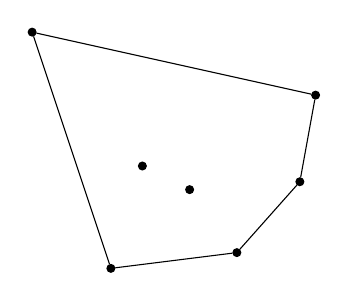
\begin{tikzpicture}\tikzset{vertex/.style = {shape=circle,draw, inner sep = 1pt, fill=black}}

		\node[vertex] (A_1) at (0,4) {};
		\node[vertex] (A_2) at (1,1) {};
		\node[vertex] (A_3) at (1.4,2.3) {};
		\node[vertex] (A_4) at (2.6,1.2) {};
		\node[vertex] (A_5) at (3.6,3.2) {};
		\node[vertex] (A_6) at (3.4,2.1) {};
		\node[vertex] (A_7) at (2,2) {};

		\draw (A_1) -- (A_2) -- (A_4) -- (A_6) -- (A_5) -- (A_1);
	\end{tikzpicture}
\end{center}

\noindent
Weźmy dwa punkty $A$, $B$ będące wierzchołkami otoczki wypukłej $Z$. Wykażemy, że dla dowolnych liczb dodatnich $k,\; l \in S$, istnieje dokładnie jeden taki punkt $X \in Z$, że
\[
AX_i = k, \quad BX_i = l. 
\]
Rozpatrzmy okrąg o środku w $A$ i promieniu $k$ oraz okrąg o środku w $B$ i promieniu $k$. Przecinają się one w co najwyżej dwóch punktach. Jeśli są to dwa różne punkty, to są symetryczne względem prostej $AB$. Cały zbiór $Z$ leży po tej samej stronie prostej $AB$, toteż co najwyżej jeden z punktów przecięcia tych okręgów należy do $Z$.

\vspace{10px}
\noindent
Zauważmy, że dla każdego $X \in Z - \{A, B\}$ liczby $AX$ i $BX$ należą do zbioru $S$. Łącząc powyższe obserwacje otrzymujemy, że liczba elementów $Z$ poza $A$ i $B$ jest nie większa niż liczba par $(k, \; l)$, gdzie $k, \; l \in S$. Stąd
\[
	10000 = |Z - \{A, B\}| \leqslant |S|^2,
\]
czyli
\[
	|S| \geqslant \sqrt{10000} = 100. 
\]
\qed

\noindent
Warto zapamiętać pojęcie otoczki wypukłej, jest ono bardzo przydatne i pozwala uniknąć dużych trudności w ścisłym opisaniu swojego rozwiązania. Niech się tylko czytelniczka/czytelnik zastanowi, jak bez pojęcia otoczki wypukłej znaleźć takie dwa punkty $A$ i~$B$, że wszystkie inne punkty zbioru $Z$ są po tej samej stronie prostej $AB$.

\vspace{5px}
\noindent
W powyższym zadaniu narzuca się analogia grafowa -- niech punkty będą wierzchołkami, a odcinki krawędziami. Jednak wtedy tracimy bardzo poważne założenie -- mianowicie, że te punkty leżą na płaszczyźnie. Jeśli widzimy, że bez tego założenia nie dałoby się rozwiązać zadania, to warto próbować je maksymalnie wykorzystać. W powyższym rozwiązaniu używamy go, aby pokazać, że odległości od $A$ i $B$ wyznaczają dokładnie jeden punkt.

\vspace{5px}
\noindent
W zadaniach z geometrii kombinatorycznej warto próbować korzystać z tego, że zadanie jest geometryczne. Może warto skorzystać z własności pól, nierówności trójkąta czy też pokolorować obszary.

\vspace{5px}



